%!TEX root = TableSummarization.tex

\section{Experiments}\label{sec:experiments}

\begin{comment} ask about below:
Additional experiments:
Maybe also good to fix mw, and show the performance with or without sampling,
and with or without a-priori (one rule per phase, for instance).
Also, would be good to see performance on increasing dataset size.
\end{comment}

\subsection{Dataset}
The dataset we use is a marketing dataset (MD), which contains demographic information about potential customers. The source of the dataset is Impact Resources, Inc., Columbus, OH (1987). A total of $N=9409$ questionnaires containing $502$ questions were 
filled out by shopping mall customers in the San Francisco Bay area. This dataset is an extract from this survey. Each tuple in the data table describes a single person. There are $14$ columns, each of which is a demographic attribute, such as annual income, Gender, marital status, age, education, and so on. Continuous values, such as income, have been bucketized in the dataset, and thus each column has upto $10$ distinct values. 

The columns (in order) are as follows:
Annual Income of Household, Sex, Marital Status, Age, Education, Occupation, Time lived in Bay Area, Dual Incomes?, Persons in Household, Persons in Household under $18$, Householder Status, Type of Home, Ethnic Classification, Language most spoken in home.

Unless otherwise specified, in all our experiments, we restrict the table to the first $7$ columns in order to make the result tables fit into the page. We set the $k$ (number of rules) parameter to $4$, and $m_w$ to $5$ for the Size weighting function, and $20$ for the Bits weighting function. 

\subsection{Qualitative Study}
We first perform a qualitative study of our Smart Drill Down system. We observe the effects of various user interface operations on our dataset, and then try out a few different weight functions to study their effects.
\subsubsection{User interface testing}
We now present the rule-based summaries displayed as a result of a few different user actions.

To begin with, the user sees an empty rule with the total number of tuples as the count. After this, suppose the user expands the rule. Then the user will see Table~\ref{table:uiexample1}. The first two new rules simply tell us that the table has $4918$ female and $4075$ male tuples. The next two rules also slightly more detailed, saying that there are $2940$ females who have been in the Bay Area for $> 10$ years, and $980$ males who have never been married and been in the Bay Are for $> 10$ years. Note that the latter two rules give very specific information which would require upto $3$ user clicks to find using Data Cube Drill-Downs, whereas our system displays that information to the user with a single click. 

Now suppose the user decides to further explore the table, by looking at education related information of females in the dataset. So the user clicks on the $\star$ in the 'Education' column of the second rule. This opens up table~\ref{table:uiexamplestar}. It shows the number of females with different levels of education, for the $4$ most frequent levels of education among females.

Instead of expanding the 'Education' column, if the user had simply expanded the third rule, it would have displayed table~\ref{table:uiexamplerule}. 

\begin{table*} 
\centering 
\begin{tabular}{| p{1.5cm} | p{1.5cm} | p{1.5cm} | p{1.5cm} | p{1.5cm} | p{1.5cm} | l | l |} 
\hline Gender & Marital Status & Age & Education & Occupation & Time in Bay Area & Count & Weight \\ \hline 
\cline{1-8} $\star$ & $\star$ & $\star$ & $\star$ & $\star$ & $\star$ & $8993$ & $0$ \\
\cline{1-1} \cline{2-2} \cline{3-3} \cline{4-4} \cline{5-5} \cline{6-6} \cline{7-8} $\triangleright$ Female & $\star$ & $\star$ & $\star$ & $\star$ & $\star$ & $4918$ & $1$ \\
\cline{1-1} \cline{2-2} \cline{3-3} \cline{4-4} \cline{5-5} \cline{6-6} \cline{7-8} $\triangleright$ Male & $\star$ & $\star$ & $\star$ & $\star$ & $\star$ & $4075$ & $1$ \\
\cline{1-1} \cline{2-2} \cline{3-3} \cline{4-4} \cline{5-5} \cline{6-6} \cline{7-8} $\triangleright$ Female & $\star$ & $\star$ & $\star$ & $\star$ & > 10 years & $2940$ & $2$ \\
\cline{1-1} \cline{2-2} \cline{3-3} \cline{4-4} \cline{5-5} \cline{6-6} \cline{7-8} $\triangleright$ Male & Never married & $\star$ & $\star$ & $\star$ & > 10 years & $980$ & $3$ \\
\hline 
\end{tabular} 
\caption{Summary after clicking on the empty rule \label{table:uiexample1}} 
\end{table*} 

\begin{table*} 
\centering 
\begin{tabular}{| p{1.5cm} | p{1.5cm} | p{1.5cm} | p{1.5cm} | p{1.5cm} | p{1.5cm} | l | l |} 
\hline Gender & Marital Status & Age & Education & Occupation & Time in Bay Area & Count & Weight \\ \hline 
\cline{1-8} $\star$ & $\star$ & $\star$ & $\star$ & $\star$ & $\star$ & $8993$ & $0$ \\
\cline{1-1} \cline{2-2} \cline{3-3} \cline{4-4} \cline{5-5} \cline{6-6} \cline{7-8} $\triangleright$ Female & $\star$ & $\star$ & $\star$ & $\star$ & $\star$ & $4918$ & $1$ \\
\cline{2-2} \cline{3-3} \cline{4-4} \cline{5-5} \cline{6-6} \cline{7-8} $\triangleright$ $\triangleright$ Female & $\star$ & $\star$ & High school & $\star$ & $\star$ & $1149$ & $2$ \\
\cline{2-2} \cline{3-3} \cline{4-4} \cline{5-5} \cline{6-6} \cline{7-8} $\triangleright$ $\triangleright$ Female & $\star$ & $\star$ & Grades 9-11 & $\star$ & $\star$ & $605$ & $2$ \\
\cline{2-2} \cline{3-3} \cline{4-4} \cline{5-5} \cline{6-6} \cline{7-8} $\triangleright$ $\triangleright$ Female & $\star$ & $\star$ & College graduate & $\star$ & $\star$ & $771$ & $2$ \\
\cline{2-2} \cline{3-3} \cline{4-4} \cline{5-5} \cline{6-6} \cline{7-8} $\triangleright$ $\triangleright$ Female & $\star$ & $\star$ & 1-3 years college & $\star$ & $\star$ & $1712$ & $2$ \\
\cline{1-1} \cline{2-2} \cline{3-3} \cline{4-4} \cline{5-5} \cline{6-6} \cline{7-8} $\triangleright$ Male & $\star$ & $\star$ & $\star$ & $\star$ & $\star$ & $4075$ & $1$ \\
\cline{1-1} \cline{2-2} \cline{3-3} \cline{4-4} \cline{5-5} \cline{6-6} \cline{7-8} $\triangleright$ Female & $\star$ & $\star$ & $\star$ & $\star$ & > 10 years & $2940$ & $2$ \\
\cline{1-1} \cline{2-2} \cline{3-3} \cline{4-4} \cline{5-5} \cline{6-6} \cline{7-8} $\triangleright$ Male & Never married & $\star$ & $\star$ & $\star$ & > 10 years & $980$ & $3$ \\
\hline 
\end{tabular} 
\caption{Star expansion on 'Education' Column \label{table:uiexamplestar}} 
\end{table*} 


\begin{table*} 
\centering 
\begin{tabular}{| p{1.5cm} | p{1.5cm} | p{1.5cm} | p{1.5cm} | p{1.5cm} | p{1.5cm} | l | l |} 
\hline Gender & Marital Status & Age & Education & Occupation & Time in Bay Area & Count & Weight \\ \hline 
\cline{1-8} $\star$ & $\star$ & $\star$ & $\star$ & $\star$ & $\star$ & $8993$ & $0$ \\
\cline{1-1} \cline{2-2} \cline{3-3} \cline{4-4} \cline{5-5} \cline{6-6} \cline{7-8} $\triangleright$ Female & $\star$ & $\star$ & $\star$ & $\star$ & $\star$ & $4918$ & $1$ \\
\cline{1-1} \cline{2-2} \cline{3-3} \cline{4-4} \cline{5-5} \cline{6-6} \cline{7-8} $\triangleright$ Male & $\star$ & $\star$ & $\star$ & $\star$ & $\star$ & $4075$ & $1$ \\
\cline{2-2} \cline{3-3} \cline{4-4} \cline{5-5} \cline{6-6} \cline{7-8} $\triangleright$ $\triangleright$ Male & Never married & $\star$ & $\star$ & $\star$ & $\star$ & $1897$ & $2$ \\
\cline{2-2} \cline{3-3} \cline{4-4} \cline{5-5} \cline{6-6} \cline{7-8} $\triangleright$ $\triangleright$ Male & Married & $\star$ & $\star$ & $\star$ & $\star$ & $1368$ & $2$ \\
\cline{2-2} \cline{3-3} \cline{4-4} \cline{5-5} \cline{6-6} \cline{7-8} $\triangleright$ $\triangleright$ Male & Never married & $\star$ & $\star$ & $\star$ & > 10 years & $980$ & $3$ \\
\cline{2-2} \cline{3-3} \cline{4-4} \cline{5-5} \cline{6-6} \cline{7-8} $\triangleright$ $\triangleright$ Male & $\star$ & $\star$ & $\star$ & $\star$ & > 10 years & $2242$ & $2$ \\
\cline{1-1} \cline{2-2} \cline{3-3} \cline{4-4} \cline{5-5} \cline{6-6} \cline{7-8} $\triangleright$ Female & $\star$ & $\star$ & $\star$ & $\star$ & > 10 years & $2940$ & $2$ \\
\hline 
\end{tabular} 
\caption{A Rule expansion \label{table:uiexamplerule}} 
\end{table*} 

\subsubsection{Weighting functions}
Our system can display optimal rule summaries using any monotonic weighting function. By default, we assign a rule weight equal to it's size. In this section, we try out a couple of other weighting functions. 

We first try the weighting function given by:
$$W(r) = \sum_{c \in C : r(c) \neq \star} \lceil \text{log}_2(|c|) \rceil$$ where $|c|$ refers to the number of distinct possible values in column $c$. This function gives higher weight to rules that have non-$\star$ values in columns that have many possible values. The rule summary for this weighting is in table~\ref{table:weigtingbitwise} (contrast with Table~\ref{table:uiexample1}). The weighting scheme gives low weight for non-$\star$ values in binary columns, like the gender column. Thus this summary instead gives us information about the Marital Status/Time in Bay Area/Occupation columns instead of the Gender column like in Table~\ref{table:uiexample1}.  

The other weighting function we try is given by:
$$W(r) = \text{Min}(0, \text{Size}(r) - 1)$$
This gives us table~\ref{table:weightingsizeminusone}. This weighting gives a $0$ weight to rules with a single non-$\star$ value, and thus forces the algorithm to finds good rules having at least $2$ non-$\star$ values. As a result, we can see that our system only displays rules having $2$ or $3$ non-$\star$ values, unlike Table~\ref{table:uiexample1} which has two rules displaying the total number of males and females, that have size $1$.

%TODO: Give application examples for different weighting functions
%TODO: Say somewhere, that we haev drop-down list of common weighting functions in the user interface, with column selects and unselects.


\begin{table*} 
\centering 
\begin{tabular}{| p{1.5cm} | p{1.5cm} | p{1.5cm} | p{1.5cm} | p{1.5cm} | p{1.5cm} | l | l |} 
\hline Gender & Marital Status & Age & Education & Occupation & Time in Bay Area & Count & Weight \\ \hline 
\cline{1-8} $\star$ & $\star$ & $\star$ & $\star$ & $\star$ & $\star$ & $8993$ & $0$ \\
\cline{1-1} \cline{2-2} \cline{3-3} \cline{4-4} \cline{5-5} \cline{6-6} \cline{7-8} $\triangleright$ $\star$ & $\star$ & $\star$ & $\star$ & $\star$ & > 10 years & $5182$ & $3$ \\
\cline{1-1} \cline{2-2} \cline{3-3} \cline{4-4} \cline{5-5} \cline{6-6} \cline{7-8} $\triangleright$ $\star$ & $\star$ & $\star$ & $\star$ & Professional / Managerial & $\star$ & $2820$ & $4$ \\
\cline{1-1} \cline{2-2} \cline{3-3} \cline{4-4} \cline{5-5} \cline{6-6} \cline{7-8} $\triangleright$ $\star$ & Never married & $\star$ & $\star$ & Student & > 10 years & $742$ & $10$ \\
\cline{1-1} \cline{2-2} \cline{3-3} \cline{4-4} \cline{5-5} \cline{6-6} \cline{7-8} $\triangleright$ $\star$ & Married & $\star$ & $\star$ & Professional / Managerial & > 10 years & $825$ & $10$ \\
\hline 
\end{tabular} 
\caption{Bits scoring\label{table:weigtingbitwise}} 
\end{table*} 

\begin{table*} 
\centering 
\begin{tabular}{| p{1.5cm} | p{1.5cm} | p{1.5cm} | p{1.5cm} | p{1.5cm} | p{1.5cm} | l | l |} 
\hline Gender & Marital Status & Age & Education & Occupation & Time in Bay Area & Count & Weight \\ \hline 
\cline{1-8} $\star$ & $\star$ & $\star$ & $\star$ & $\star$ & $\star$ & $8993$ & $0$ \\
\cline{1-1} \cline{2-2} \cline{3-3} \cline{4-4} \cline{5-5} \cline{6-6} \cline{7-8} $\triangleright$ Female & $\star$ & $\star$ & $\star$ & $\star$ & > 10 years & $2940$ & $1$ \\
\cline{1-1} \cline{2-2} \cline{3-3} \cline{4-4} \cline{5-5} \cline{6-6} \cline{7-8} $\triangleright$ Male & Never married & $\star$ & $\star$ & $\star$ & > 10 years & $980$ & $2$ \\
\cline{1-1} \cline{2-2} \cline{3-3} \cline{4-4} \cline{5-5} \cline{6-6} \cline{7-8} $\triangleright$ Female & Married & $\star$ & $\star$ & $\star$ & > 10 years & $1230$ & $2$ \\
\cline{1-1} \cline{2-2} \cline{3-3} \cline{4-4} \cline{5-5} \cline{6-6} \cline{7-8} $\triangleright$ Male & Married & $\star$ & $\star$ & $\star$ & > 10 years & $823$ & $2$ \\
\hline 
\end{tabular} 
\caption{Size minus one weighting \label{table:weightingsizeminusone}} 
\end{table*}  

\subsection{Quantitative Study}
The performance of our algorithm depends on various parameters, such as $m_w$ (the max weight) and $minSS$ (minimum required sample size). In this section, we study the effects of these parameters on the computation time and accuracy of our algorithm. 

\subsubsection{Effects of $m_w$}
Our algorithm for finding the best marginal rule (Algorithm~\ref{algo:best-marginal-rule}) takes an input parameter called $m_w$. The algorithm is guaranteed to find the best marginal rule as long as it's weight is $\leq m_w$, but runs faster for smaller values of $m_w$. In this section, we study the effect of varying $m_w$ on the speed of our algorithm. Our system is run on a Dell XPS L702X laptop with 6GB RAM and an Intel i5 2.30GHz processor.

We consider a weighting function $W$, and a value of $m_w$. For that value of the $W$ and $m_w$ parameters, we find the time taken for expanding the empty rule. We repeat this procedure $10$ times and take the average value of the running times across the $10$ iterations. This time is plotted against $m_w$, for $W(r) = \text{Size}(r)$ and $W(r) = \sum_{c \in C : r(c) \neq \star} \lceil \text{log}_2(|c|) \rceil$ in Figure~\ref{fig:mw_speed}. The figure shows that running time seems to be approximately linear in $m_w$. 

The value of $m_w$ required to ensure a correct answer is equal to the maximum weight of a selected rule. Thus for size scoring, according to Table~\ref{table:uiexample1}, we require $m_w \geq 3$. For the second weighting function, according to Table~\ref{table:weigtingbitwise}, the minimum required value of $m_w$ is $10$. At these values of $m_w$, we see that the expansion takes $1.5$ seconds and about $0.25$ seconds respectively. Of course, the minimum value of $m_w$ we can use is not known to us beforehand. But even if we use more conservative values of $m_w$, say $6$ and $20$ respectively, the running times are about $1.5$ and $0.5$ seconds respectively.

\begin{figure}
\hspace{-20pt}
  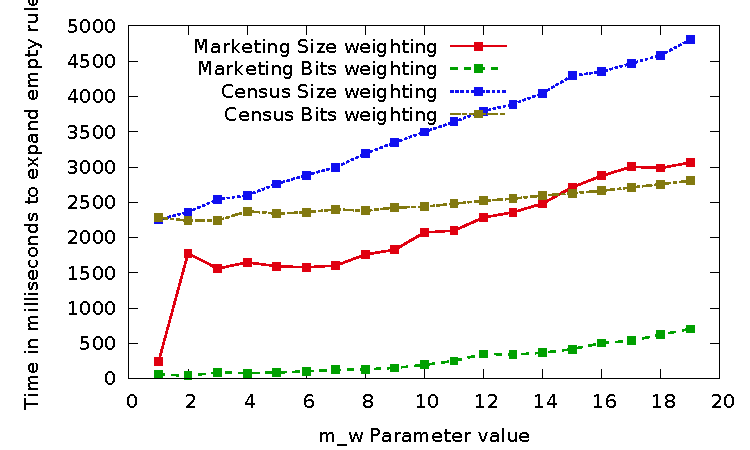
\includegraphics[height=2in]{graphs/mw_speed.pdf}%change height to 2 inch for actual paper, 5 inch for single column
\vspace{-10pt}
  \caption{Running time for different values of parameter $m_w$ \label{fig:mw_speed}}
\vspace{-13pt}
\end{figure}

\subsubsection{Effects of $minSS$}
We now study the effects of the sampling parameter $minSS$. This parameter tells the SampleHandler the minimum sample size on which we run Algorithm~\ref{algo:best-rule-set}.   Higher values of $minSS$ cause our system to use bigger samples, which increases the accuracy of count estimates for displayed rules, but also correspondingly increases computation time. 

We consider one value of $minSS$ and one weight function $W$ at a time. For those values of $minSS$ and $W$, we drill down on the empty rule and measure the time taken for this operation. We also measure the percent error in the estimated counts of the displayed rules. That is, for each displayed rule $r$, if the displayed (estimated) count if $c_1$ and the actual count (computed separately on the entire table) is $c_2$, then the percent error for rule $r$ is $\frac{100 \times |c_1-c_2|}{c_2}$. We consider the average of percent errors over all displayed rules. For each value of $minSS$ and $W$, we drill down on the empty rule and find the computation time and percent error $50$ times, and take the average value for time and error over those $50$ iterations. This average time is plotted against $minSS$, for $W(r) = \text{Size}(r)$ and $W(r) = \sum_{c \in C : r(c) \neq \star} \lceil \text{log}_2(|c|) \rceil$ in Figure~\ref{fig:minSS_speed}. The average percent error is plotted against $minSS$, for $W(r) = \text{Size}(r)$ and $W(r) = \sum_{c \in C : r(c) \neq \star} \lceil \text{log}_2(|c|) \rceil$ in Figure~\ref{fig:minSS_error_percent}. 

The computation time increases approximately linearly with parameter $minSS$. This is expected, because Algorithm~\ref{algo:best-rule-set} makes a constant number of passes over the entire sample, and each pass takes time linear in the size of the sample. The percent error decreases approximately as $\frac{1}{\sqrt{minSS}}$, which is again expected because the standard deviation of estimated $Count$ is approximately inversely proportional to the square root of sample size.

In addition, we measure the number of incorrect rules per iteration. If the correct set of rules to display is $r_1, r_2, r_3$ and the displayed set is $r_1, r_3, r_4$ then that means there is one incorrect rule. We find the number of incorrect displayed rules across $50$ iterations, and display the average value in Figure~\ref{fig:minSS_error_rule}. This number is almost always $0$ for the Size weighting function, and between $1$ and $2$ for the Bits weighting function. Note that even when we display an `incorrect' rule, it is usually the $5^{th}$ or $6^{th}$ best rule instead of one of the top $4$ rules, which still results in a reasonably good summary of the table.

\begin{figure}
\hspace{-20pt}
  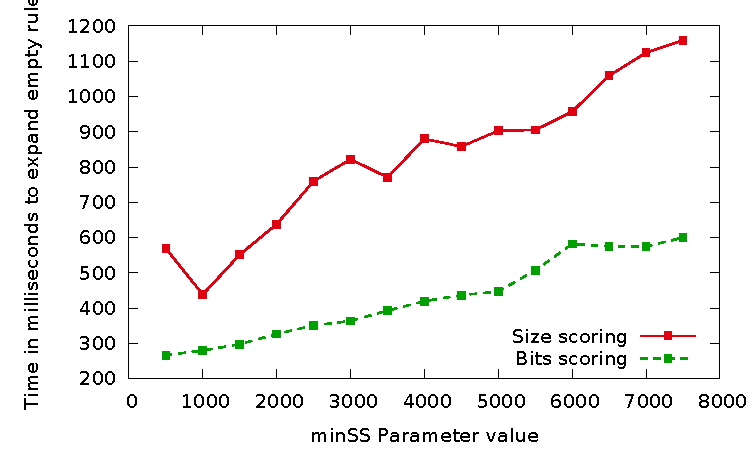
\includegraphics[height=2in]{graphs/minSS_speed.pdf}%change height to 2 inch for actual paper, 5 inch for single column
\vspace{-10pt}
  \caption{Running time for different values of parameter $minSS$ \label{fig:minSS_speed}}
\vspace{-13pt}
\end{figure}

\begin{figure}
\hspace{-20pt}
  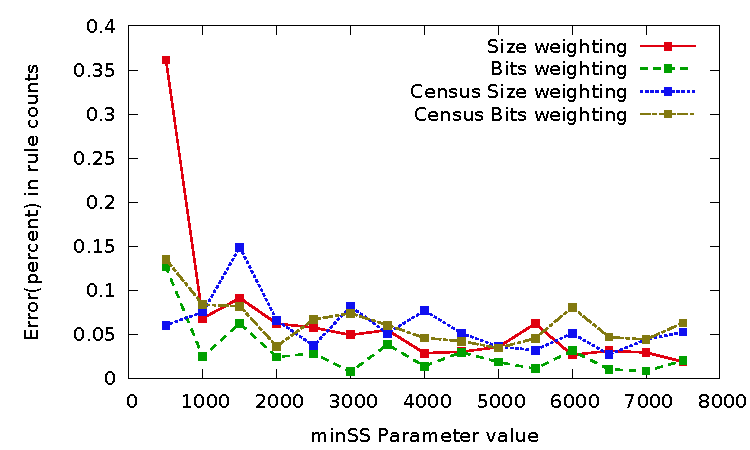
\includegraphics[height=2in]{graphs/minSS_error_percent.pdf}%change height to 2 inch for actual paper, 5 inch for single column
\vspace{-10pt}
  \caption{Error in Count for different values of parameter $minSS$ \label{fig:minSS_error_percent}}
\vspace{-13pt}
\end{figure}

\begin{figure}
\hspace{-20pt}
  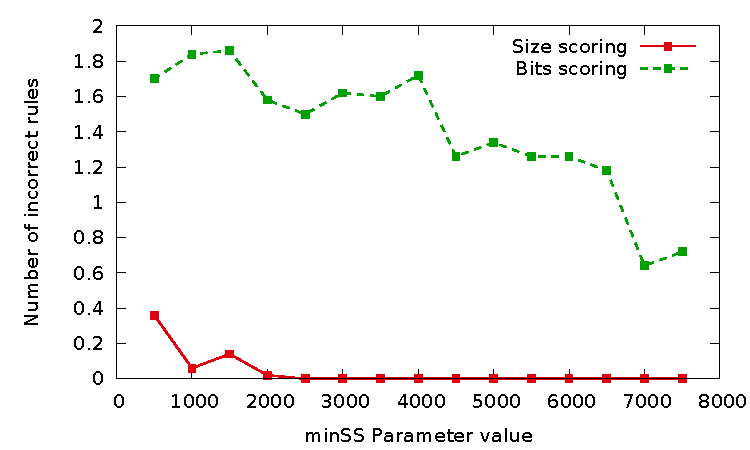
\includegraphics[height=2in]{graphs/minSS_error_rule.pdf}%change height to 2 inch for actual paper, 5 inch for single column
\vspace{-10pt}
\caption{Average number of incorrect rules for different values of parameter $minSS$ \label{fig:minSS_error_rule}}
\vspace{-13pt}
\end{figure}